
\documentclass[
	11pt, % Set the default font size, options include: 8pt, 9pt, 10pt, 11pt, 12pt, 14pt, 17pt, 20pt
	%t, % Uncomment to vertically align all slide content to the top of the slide, rather than the default centered
	% aspectratio=169, % Uncomment to set the aspect ratio to a 16:9 ratio which matches the aspect ratio of 1080p and 4K screens and projectors
]{beamer}

\graphicspath{{Images/}{./}} % Specifies where to look for included images (trailing slash required)

\usepackage{booktabs} % Allows the use of \toprule, \midrule and \bottomrule for better rules in tables

%----------------------------------------------------------------------------------------
%	SELECT LAYOUT THEME
%----------------------------------------------------------------------------------------

% Beamer comes with a number of default layout themes which change the colors and layouts of slides. Below is a list of all themes available, uncomment each in turn to see what they look like.

% \usetheme{default}
% \usetheme{AnnArbor}
% \usetheme{Antibes}
% \usetheme{Bergen}
% \usetheme{Berkeley}
% \usetheme{Berlin}
% \usetheme{Boadilla}
% \usetheme{CambridgeUS}
% \usetheme{Copenhagen}
% \usetheme{Darmstadt}
% \usetheme{Dresden}
\usetheme{Frankfurt}
% \usetheme{Goettingen}
% \usetheme{Hannover}
% \usetheme{Ilmenau}
% \usetheme{JuanLesPins}
% \usetheme{Luebeck}
% \usetheme{Madrid}
% \usetheme{Malmoe}
% \usetheme{Marburg}
% \usetheme{Montpellier}
% \usetheme{PaloAlto}
% \usetheme{Pittsburgh}
% \usetheme{Rochester}
% \usetheme{Singapore}
% \usetheme{Szeged}
% \usetheme{Warsaw}

%----------------------------------------------------------------------------------------
%	SELECT COLOR THEME
%----------------------------------------------------------------------------------------

% Beamer comes with a number of color themes that can be applied to any layout theme to change its colors. Uncomment each of these in turn to see how they change the colors of your selected layout theme.

% \usecolortheme{albatross}
\usecolortheme{beaver} % okay
% \usecolortheme{beetle}
% \usecolortheme{crane} % good
% \usecolortheme{dolphin}
% \usecolortheme{dove}
% \usecolortheme{fly}
% \usecolortheme{lily}
% \usecolortheme{monarca}
% \usecolortheme{seagull}
% \usecolortheme{seahorse}
% \usecolortheme{spruce}
% \usecolortheme{whale}
% \usecolortheme{wolverine} % okay

%----------------------------------------------------------------------------------------
%	SELECT FONT THEME & FONTS
%----------------------------------------------------------------------------------------

% Beamer comes with several font themes to easily change the fonts used in various parts of the presentation. Review the comments beside each one to decide if you would like to use it. Note that additional options can be specified for several of these font themes, consult the beamer documentation for more information.

\usefonttheme{default} % Typeset using the default sans serif font
% \usefonttheme{serif} % Typeset using the default serif font (make sure a sans font isn't being set as the default font if you use this option!)
% \usefonttheme{structurebold} % Typeset important structure text (titles, headlines, footlines, sidebar, etc) in bold
% \usefonttheme{structureitalicserif} % Typeset important structure text (titles, headlines, footlines, sidebar, etc) in italic serif
% \usefonttheme{structuresmallcapsserif} % Typeset important structure text (titles, headlines, footlines, sidebar, etc) in small caps serif

%------------------------------------------------

% \usepackage{mathptmx} % Use the Times font for serif text
% \usepackage{palatino} % Use the Palatino font for serif text

% \usepackage{helvet} % Use the Helvetica font for sans serif text
% \usepackage[default]{opensans} % Use the Open Sans font for sans serif text
\usepackage[default]{FiraSans} % Use the Fira Sans font for sans serif text
% \usepackage[default]{lato} % Use the Lato font for sans serif text

%----------------------------------------------------------------------------------------
%	SELECT INNER THEME
%----------------------------------------------------------------------------------------

% Inner themes change the styling of internal slide elements, for example: bullet points, blocks, bibliography entries, title pages, theorems, etc. Uncomment each theme in turn to see what changes it makes to your presentation.

%\useinnertheme{default}
\useinnertheme{circles}
% \useinnertheme{rectangles}
% \useinnertheme{rounded}
% \useinnertheme{inmargin}

%----------------------------------------------------------------------------------------
%	SELECT OUTER THEME
%----------------------------------------------------------------------------------------

% Outer themes change the overall layout of slides, such as: header and footer lines, sidebars and slide titles. Uncomment each theme in turn to see what changes it makes to your presentation.

% \useoutertheme{default}
% \useoutertheme{infolines}
% \useoutertheme{miniframes}
\useoutertheme{smoothbars}
% \useoutertheme{sidebar}
% \useoutertheme{split}
% \useoutertheme{shadow}
% \useoutertheme{tree}
% \useoutertheme{smoothtree}

%\setbeamertemplate{footline} % Uncomment this line to remove the footer line in all slides
% \setbeamertemplate{footline}[page number] % Uncomment this line to replace the footer line in all slides with a simple slide count

% \setbeamertemplate{navigation symbols}{} % Uncomment this line to remove the navigation symbols from the bottom of all slides

%----------------------------------------------------------------------------------------
%	PRESENTATION INFORMATION
%----------------------------------------------------------------------------------------

\title[MTH689A]{Influential Observations in Linear Regression} % The short title in the optional parameter appears at the bottom of every slide, the full title in the main parameter is only on the title page

\subtitle{Author: R. Dennis Cook} % Presentation subtitle, remove this command if a subtitle isn't required

\author[Sunil Dhaka]{Sunil Dhaka} % Presenter name(s), the optional parameter can contain a shortened version to appear on the bottom of every slide, while the main parameter will appear on the title slide

\institute[IITK]{Indian Institute of Technology, Kanpur \\ \smallskip \textit{sunild@iitk.ac.in}} % Your institution, the optional parameter can be used for the institution shorthand and will appear on the bottom of every slide after author names, while the required parameter is used on the title slide and can include your email address or additional information on separate lines

\date[\today]{Linear and Non-Linear Models \\ \today} % Presentation date or conference/meeting name, the optional parameter can contain a shortened version to appear on the bottom of every slide, while the required parameter value is output to the title slide

%----------------------------------------------------------------------------------------
\begin{document}
%page-1
\begin{frame}
	\maketitle
\end{frame}
% page-2
\begin{frame}
	\frametitle{Table of Contents}
	\tableofcontents
\end{frame}

\section{Introduction}

\begin{frame}
	\frametitle{Definitions}
	\begin{itemize}
		\item An \textbf{outlier} is a data point whose response y does not follow the general trend of the rest of the data.
		\pause
		\item A data point has \textbf{high leverage} if it has "extreme" predictor x values.
		\pause
		\item A data point is \textbf{influential} if it unduly influences any part of a regression analysis, such as the predicted responses, the
		estimated slope coefficients, or the hypothesis test results.
		\pause
		\begin{itemize}
			\item Outliers and high leverage data points have the potential to be influential, but we generally have to investigate further to determine whether or not they are actually influential.
			\item A data point is influential or not depends on the observed value of reponse and predictor of point 
		\end{itemize}
	\end{itemize}
\end{frame}


\begin{frame}[allowframebreaks]
	\frametitle{Example}
	\begin{figure}
		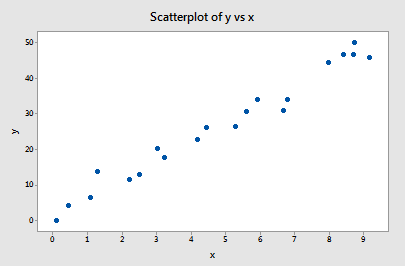
\includegraphics[scale=0.9]{influ_scatter_01.png}
	\end{figure}
	\begin{figure}
		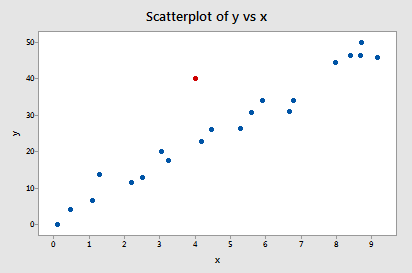
\includegraphics[scale=0.9]{influ_scatter_02.png}
	\end{figure} 
	\begin{figure}
		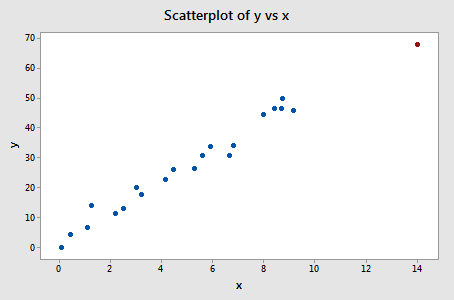
\includegraphics[scale=0.8]{influ_scatter_06.png}
	\end{figure} 
	\begin{figure}
		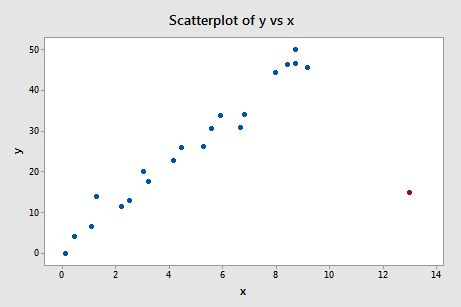
\includegraphics[scale=0.8]{influ_scatter_09.png}
	\end{figure}
\end{frame}

\begin{frame}
	\frametitle{Remarks}
	\begin{itemize}
		\item the easy situation occurs for SLR, which can be visualized in 2D scatter plots
		\pause
		\item do not have that luxury in the case of MLR
		\pause
		\item we have to rely on various measures to help us determine whether a data point is an outlier, high leverage, or both
		\pause
		\item then need to see if the points are actually influential
		\pause
		\item after that have to decide whether to include or exclude such observations
		\pause
		\begin{itemize}
				\item must have a good, \textbf{objective} reason for deleting data points, then justify it with results
				\pause
				\item common sense and knowledge about the situation matters
		\end{itemize}	
	\end{itemize}
\end{frame}

\section{Identifying high leverage points}

\begin{frame}[allowframebreaks]
	\frametitle{Setup and notations}
	\begin{itemize}
		
		\item consider standard full rank model
		\begin{equation*}
			\mathbf{Y}=\mathbf{X\beta}+\mathbf{e}
		\end{equation*}
		\item estimated coefficients
		\begin{equation*}
			\mathbf{\hat{\beta}}=\mathbf{(X^{'}X)^{-1}X^{'}Y}
		\end{equation*}
		\item hat matrix
		\begin{equation*}
			V=(v_{ij})=\mathbf{X(X^{'}X)^{-1}X^{'}}
		\end{equation*}
		\item predicted values: $\mathbf{\hat{Y}}=(y_i)=\mathbf{X\hat{\beta}}=\mathbf{VY}$
		\begin{equation*}
			Var(\mathbf{\hat{Y}})=\sigma^2\mathbf{V}
		\end{equation*}
		\item residuals: $\mathbf{R}=(r_i)=(\mathbf{Y-\hat{Y}})=(\mathbf{I-V})Y$
		\begin{equation*}
			Var(\mathbf{R})=\sigma^2(\mathbf{I-V})
		\end{equation*}
		\end{itemize}
\end{frame}

\begin{frame}[allowframebreaks]
	\frametitle{Detecting high leverage points}
	\begin{itemize}
		\item why bother? in certain situations they may highly influence the estimated regression function, so need to identify
		\item leverage $v_{ii}$: 
		\begin{itemize}
			\item $\hat{y_i}=v_{i1}y_1+\ldots+\mathbf{v_{ii}y_i}+\ldots+v_{in}y_n$
			\item it is $i^{th}$ row element of $\mathbf{VY}$ matrix
			\item quantifies the influence that the observed response $y_i$ has on its predicted value $\hat{y_i}$
		\end{itemize}
		% quantifies the influence that the observed response $y_i$ has on its predicted value $\hat{y_i}$
	% 	That is, if
	% 	is small,
	%    then the observed response
	% 	plays only a small role in the value of the predicted response . On the other hand, if
	% 	is
	%    large, then the observed response
	% 	plays a large role in the value of the predicted response . It's for this reason that the
	%    are called the "leverages." 
		\item why they are called leverages?
		\begin{itemize}
			\item $v_{ii}$ quantifies how far away the $i^{th}$ $x$ value is from the rest of the $x$ values
		   \item $0 \leq v_{ii} \leq 1$
		   \item $\sum_{i=1}^n v_{ii}=p$, reason?
		\end{itemize}
		\item we select points with large leverage values as potential influential points
		\item what value should be considered large? 
		\begin{itemize}
			\item though the cut-off value depends on the situation and the analyst
			\item common rule: more than 3 times larger than the mean leverage value
			\begin{equation*}
				v_{ii}>3\frac{\sum_{i=1}^n v_{ii}}{n}=3\frac{p}{n}
			\end{equation*}
		\end{itemize}
	\end{itemize}
\end{frame}

\begin{frame}[allowframebreaks]
	\frametitle{High leverage point example}
	\begin{figure}
		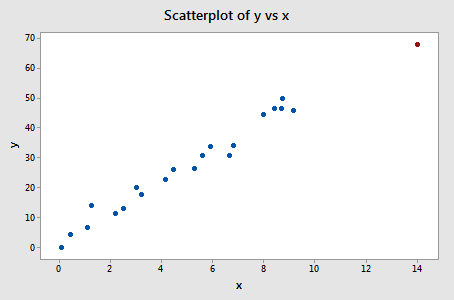
\includegraphics[scale=0.8]{influ_scatter_06.png}
	\end{figure}


	\begin{figure}
		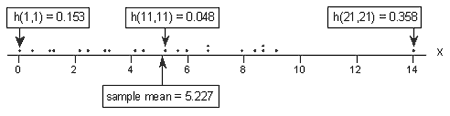
\includegraphics[scale=0.5]{dotplot2_plot.png}
	\end{figure}

	\begin{itemize}
		\item $n=21$ and $p=2$ (SLR); flag value $3\frac{p}{n}=0.286$
		\item red point($x=14,y=68$) has leverage value $=0.358$
		\item the data point \textbf{should} be flagged as high leverage point
		\item leverages only take into account the extremeness of the $x$ values, but a high leverage
		observation may or may not actually be influential
	\end{itemize}
\end{frame}

\section{Identifying outliers}

\begin{frame}[allowframebreaks]
	\frametitle{Outlier detection}
	\begin{itemize}
		\item residuals can help in detecting outliers as measures the difference between the observed and
		predicted responses
		% teach: talk about that outlier example plot from previous slides, how that gap/difference between the difference between the observed and prediccted might indicate outlier 
		% always can not plot and see whether it is an outlier or not
		\item why need studentized residuals?
		\begin{itemize}
			\item the major problem with ordinary residuals is that their magnitude depends on the units of measurement,
			thereby making it difficult to use the residuals as a way of detecting unusual y values
		\end{itemize}
		\begin{equation*}
			t_i=\frac{r_i}{sd(r_i)}=\frac{r_i}{\sqrt{MSE(1-v_{ii})}}
		\end{equation*}
		\begin{itemize}
			\item depends on the leverage $h_{ii}$
		\end{itemize}
		\item how to use it for outlier detection?
		\begin{itemize}
			\item  they quantify how large the residuals are in standard deviation
			units
			\item studentized residual that is larger than 3 (in absolute value) is generally decided as
			outlier
			\item again depends on the situation and the analyst
			% teach: suppose there are std residual values that are around 2.5 to 3, and one is 3.1 ; then should we choose it as an outlier
		\end{itemize}
	\end{itemize}
	\begin{figure}
		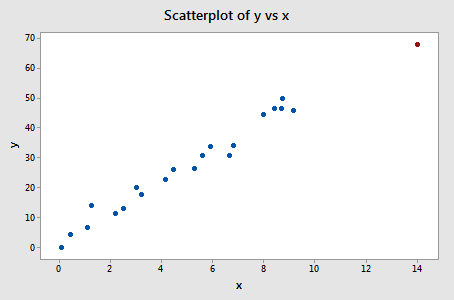
\includegraphics[scale=0.8]{influ_scatter_06.png}
	\end{figure} 
	\begin{itemize}
		\item std residual for red point $=3.68 > 3$
		\item deemed as an outlier, further investigation to decide whether it is an influential point or not
	\end{itemize}
\end{frame}

\begin{frame}
	\frametitle{Intermission}
	\begin{itemize}
		% needs to be edited
		\item When trying to identify outliers, one problem that can arise is when there is a potential outlier that influences the
		regression model to such an extent that the estimated regression function is "pulled" towards the potential outlier, so that it
		isn't flagged as an outlier using the standardized residual criterion.
		\item To address this issue, deleted residuals offer an alternative criterion for identifying outliers.
		\item The basic idea is to delete the observations one at a time, each time refitting the
		regression model on the remaining $n-1$ observations. Then, we compare the observed response values to their fitted values
		based on the models with the ith observation deleted.
		% \begin{equation*}
		% 	t_i=\frac{r_i}{s\sqrt{(1-v_{ii})}}
		% \end{equation*}
	\end{itemize}
\end{frame}

\section{Influential observations}

\begin{frame}
	\frametitle{Cooks distance measure}
	\begin{itemize}
		\item the influence of the $i_{th}$	data point be judged by using the distance measure
		\begin{equation}
			D_i=\frac{(\hat{\beta}-\hat{\beta_{(i)}})^{'}(X^{'}X)(\hat{\beta}-\hat{\beta_{(i)}})}{ps^2}
		\end{equation}
		here, $s^2=MSE=\frac{R^{'}R}{(n-p)}$
		\item large value of $D_i$ indicates that the associated $i^{th}$ point has a strong influence on the estimate of regression parameters $\beta$
		\item magnitude of the distance between $\hat{\beta}$ and $\hat{\beta_{(i)}}$
		\begin{itemize}
				\item compare $D_i$ value to probability points of $F_{p,n-p,ncp=0}$
				\item equivalent to finding level of the confidence ellipsoid
% 				% center at \hat{\beta} and passign through beta_{(i)}
		\end{itemize}
	\end{itemize}
\end{frame}
	
\begin{frame}
	\frametitle{Alternative form}
	\begin{itemize}
		\item using $\hat{\beta}-\hat{\beta_{(i)}}=\frac{(X^{'}X)^{-1}x_ir_i}{1-v_{ii}}$ result, we get 
		\begin{equation*}
			D_i=\frac{t_i^2w_i}{p}
		\end{equation*}
		\item $D_i$ can be large if either $t_i^2$ or $w_i$ is large
		\item $t_i=\frac{r_i}{s\sqrt{(1-v_{ii})}}$, is $i_{th}$ deleted studentized residual
		\item it depends on the residual, measures outlier properties of the observation
		\item $w_i=\frac{v_{ii}}{(1-v_{ii})}$, ratio of the variance of the
		$i_{th}$ predicted value and the variance of the $i_{th}$ residual
		\item it also depends on the leverage of the observation, measures the location of the $i_{th}$ observation
		\item Cook's distance incorporates both outlier($y$ value) and high leverage($x$ value) properties of an observation
	\end{itemize}
\end{frame}

\begin{frame}
	\frametitle{Using Cook's distance measures}
	\begin{itemize}
		\item for MLR models we need to rely on guidelines/rules for deciding when a Cook's distance
		measure is large enough to deem a data point as influential observation
		\item common rule:
		\begin{itemize}
			\item $D_i > 0.5$ then may be influential, but needs further investigation
			\item $D_i > 1$, quite likely to be influential
			\item $D_i >> 1$, almost certainly influential
		\end{itemize}
	\end{itemize}
\end{frame}

\begin{frame}[allowframebreaks]
	\frametitle{Examples}
	R scripts
\end{frame}

\section{Consequences of deleting an observation}

\begin{frame}[allowframebreaks]
	\frametitle{Residual Correlation}
	% WHY?????????????
	\begin{block}
		{Goal:} to find out $t_{j(i)}$ that is $\mathbf{j_{th}}$(not $i_{th}$) deleted studentized residual based on the data set with $i_{th}$ point removed, 
	\end{block}
		
	\begin{itemize}
		\item consider
		\begin{equation}
			v_{kl}=x_k^{'}(X_{(i)}^{'}X_{(i)})^{-1}x_l^{'}
		\end{equation}
		here, $X_{(i)}^{'}X_{(i)}=X^{'}X-x_ix_i^{'}$ and $x_i$ is $i_{th}$ row
		\item using general identity
		\begin{equation*}
			\left[B+uz^{'}\right]^{-1}=B^-1-\frac{B^-1uz^{'}B^-1}{1+u^{'}B^{-1}z}
		\end{equation*}
		after using this on eq(1) expressions and a bit algebra,
		\begin{align}
			v_{kl}&=v_{kl(i)}-\frac{v_{ki(i)}v_{li(i)}}{1+v_{ii}}\\
			v_{kl(i)}&=v_{kl}+\frac{v_{ki}v_{li}}{1-v_{ii}}
		\end{align}
		
		\item other two results that are used to get $t_{j(i)}$
		\begin{align}
			\hat{\beta}-\hat{\beta_{(i)}}&=\frac{(X^{'}X)^{-1}x_ir_i}{1-v_{ii}}\\
			(n-p)s^2&=(n-p-1)s_{(i)}^2+\frac{r_i^2}{1-v_{ii}}
		\end{align}
		\item $\rho_{ij}$: residual correlation in \textbf{full} dataset
		\item ratio $w_{j(i)}$, when $j \neq i$
		\begin{equation}
			\frac{v_{jj(i)}}{1-v_{jj(i)}}=\frac{v_{jj}(1-\rho_{ij}^2)+\rho_{ij}^2}{(1-v_{jj}(1-\rho_{ij}^2))}
		\end{equation}
		\begin{itemize}
			\item ratio will be large if either $v_{jj}$ or $\rho_{ij}^2$ is large
			\item high $v_{jj}$ would have been detected in the full data analysis
			\item now if the ratio is high, it must be due to large correlation between $i_{th}$ and $j_{th}$ residuals in full dataset
			\item and if $\rho_{ij}$ is negligible then $w_{j(i)}=w_{j}$
		\end{itemize}
		\item using results from eq(2)-(5), and with lot more algebra we get 
		\begin{equation}
			t_{j(i)}^2=\frac{(n-p-1)(t_j-\rho_{ij}t_i)^2}{(n-p-t_i^2)(1-\rho_{ij}^2)}
		\end{equation}
		\begin{itemize}
			\item if residual correlation $\rho_{ij}$ is negligible, and $t_i > 1$, then for all remaining deleted studentized residuals will increase
			\item if $\rho_{ij}$ is large, then $j_{th}$ deleted studentized residuals increases substantially then $i_{th}$ point is deleted
		\end{itemize}
		\item note that both expressions of $w_{j(i)}$ and $t_{j(i)}^2$ are in terms of full dataset
		\item their product gives Cook's distance measure
	\end{itemize}
\end{frame}

\begin{frame}
	\frametitle{Paper Example}
	\begin{itemize}
		\item available in R as \textbf{stack}, multipler outlier example
		\item Number of Observations: 21
		\item Number of Variables: 4
		\item Variables:
		\begin{itemize}
			\item y: STACKLOSS, x: AIRFLOW, WATERTEMP, ACIDCONC
		\end{itemize}
		\item model setup: from Daniel and Wood (1971) 
		\begin{itemize}
			\item found 4 outliers: (1,3,4,21)
			\item model containes a linear and quadratic term of AIRFLOW
			\item a linear term for WATERTEMP
			\item ACIDCONC is not needed for prediction
		\end{itemize}
		\item R script
	\end{itemize}	
\end{frame}

\begin{frame} % Use [allowframebreaks] to allow automatic splitting across slides if the content is too long
	\frametitle{References}
	
	\begin{thebibliography}{99} % Beamer does not support BibTeX so references must be inserted manually as below, you may need to use multiple columns and/or reduce the font size further if you have many references
		\footnotesize % Reduce the font size in the bibliography
		\bibitem[Cook, 1979]{p}
			R. Dennis Cook (1979)
			\newblock Influential Observations in Linear Regression
			\newblock \emph{Journal of the American Statistical Association} 74(365), 169 -- 174.
	\end{thebibliography}
\end{frame}

\begin{frame}[plain] % The optional argument 'plain' hides the headline and footline
	\begin{center}
		{\Huge The End}
		
		\bigskip\bigskip % Vertical whitespace
		
		{\LARGE Questions? Comments?}
	\end{center}
\end{frame}

\end{document}